The problem of taxonomy classification of product titles is central to an e-commerce organization. 
Large online e-commerce companies usually obtain millions of new listing feeds per month from several hundred merchants subscribed to use proprietary ``publish $\rightarrow$ search $\rightarrow$ buy'' platforms specific to each of these companies. 
The ease of use, control on data quality and organization and functionality of these platforms are the key factors for differentiating the success of the revenue generation model for the companies.

The sale of product listings within an e-commerce platform is critically dependent upon end users being able to search for the correct product using some minimal to advanced search functionality provided by the developers of the platform. 
In this paper we differentiate products from product listings using a simple example. 
Consider a product with a title of ``\textit{Wilson tennis racket Level 3 signed by Federer}''. 
Merchant \textbf{A} can list this product with a title of ``\textit{Wilson tennis racquet Level 3 Roger Federer}''' and with a list price of \$80 while merchant \textbf{B} can list the same product with its original title but with a list price of \$72.
The e-commerce platform keeps track of these two product items as two different listings although they are the same product after some title text disambiguation.
Similar examples occur in thousands for product titles having the same title text but differing in price and/or other fields.
Title text disambiguation in absence of any global identifier for products is also a core-problem in e-commerce platforms that follow an online marketplace model, but we do not address that problem here.
In this paper, we will refer to product listings as listings henceforth. 

Most e-commerce companies keep track of high Gross Merchandise Sales (GMS) products and tune search results to queries conditional on this and other clickstream features as well as several other content specific features.
One such critical feature is the taxonomy classification of listings.
On a web search platform, categories of search results have already been used to improve web query classification \cite{Ganti10} and such kind of query classifications are also very useful for product search engines. 
In this paper, we focus on taxonomy classifications of listings in order to solve problems arising in the  scenario described in Fig. .

\begin{figure}[t!]
\centering
\subfloat[{BU1 branch stats}]{\label{Figure_BU1-branches}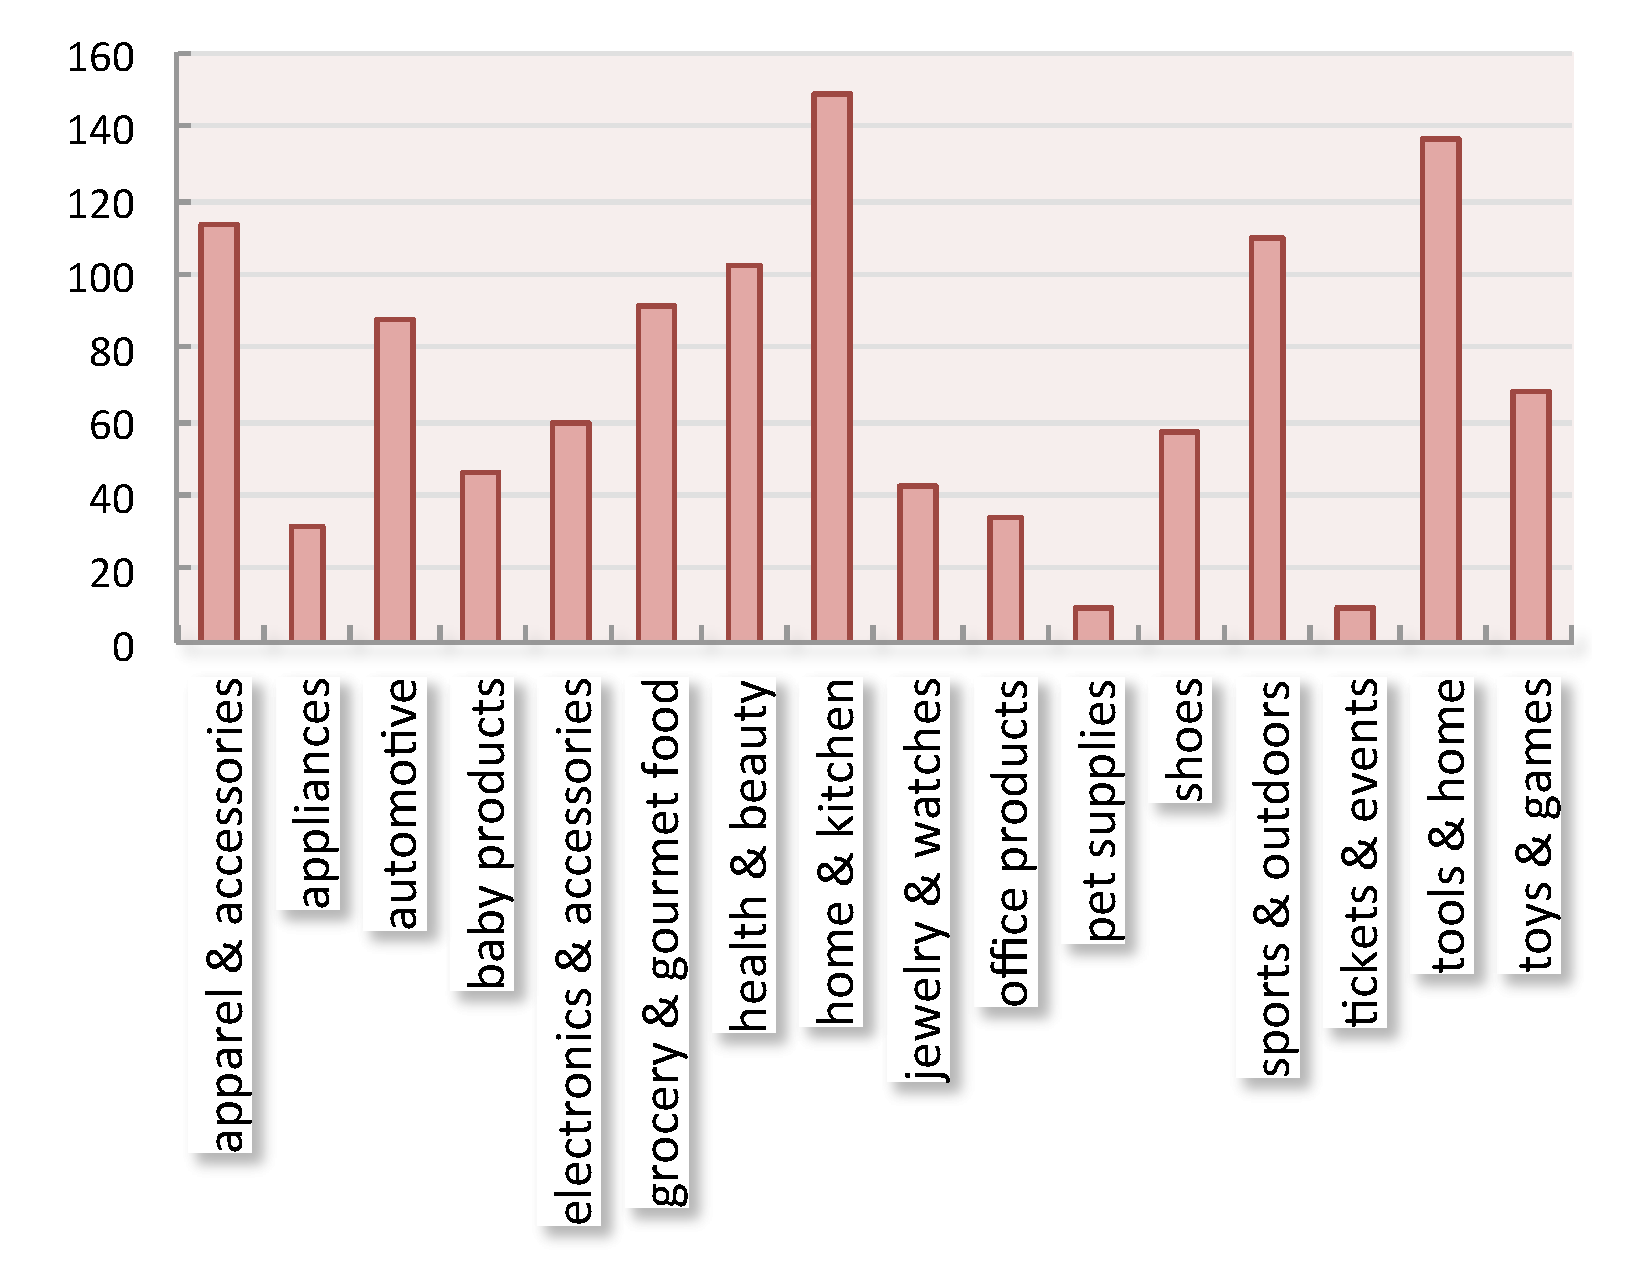
\includegraphics[width=0.32\textwidth]{images/BU1-branches}} \hspace{0.01cm}
\subfloat[{AmazonJulian branch stats}]{\label{Figure_amazonj-branches}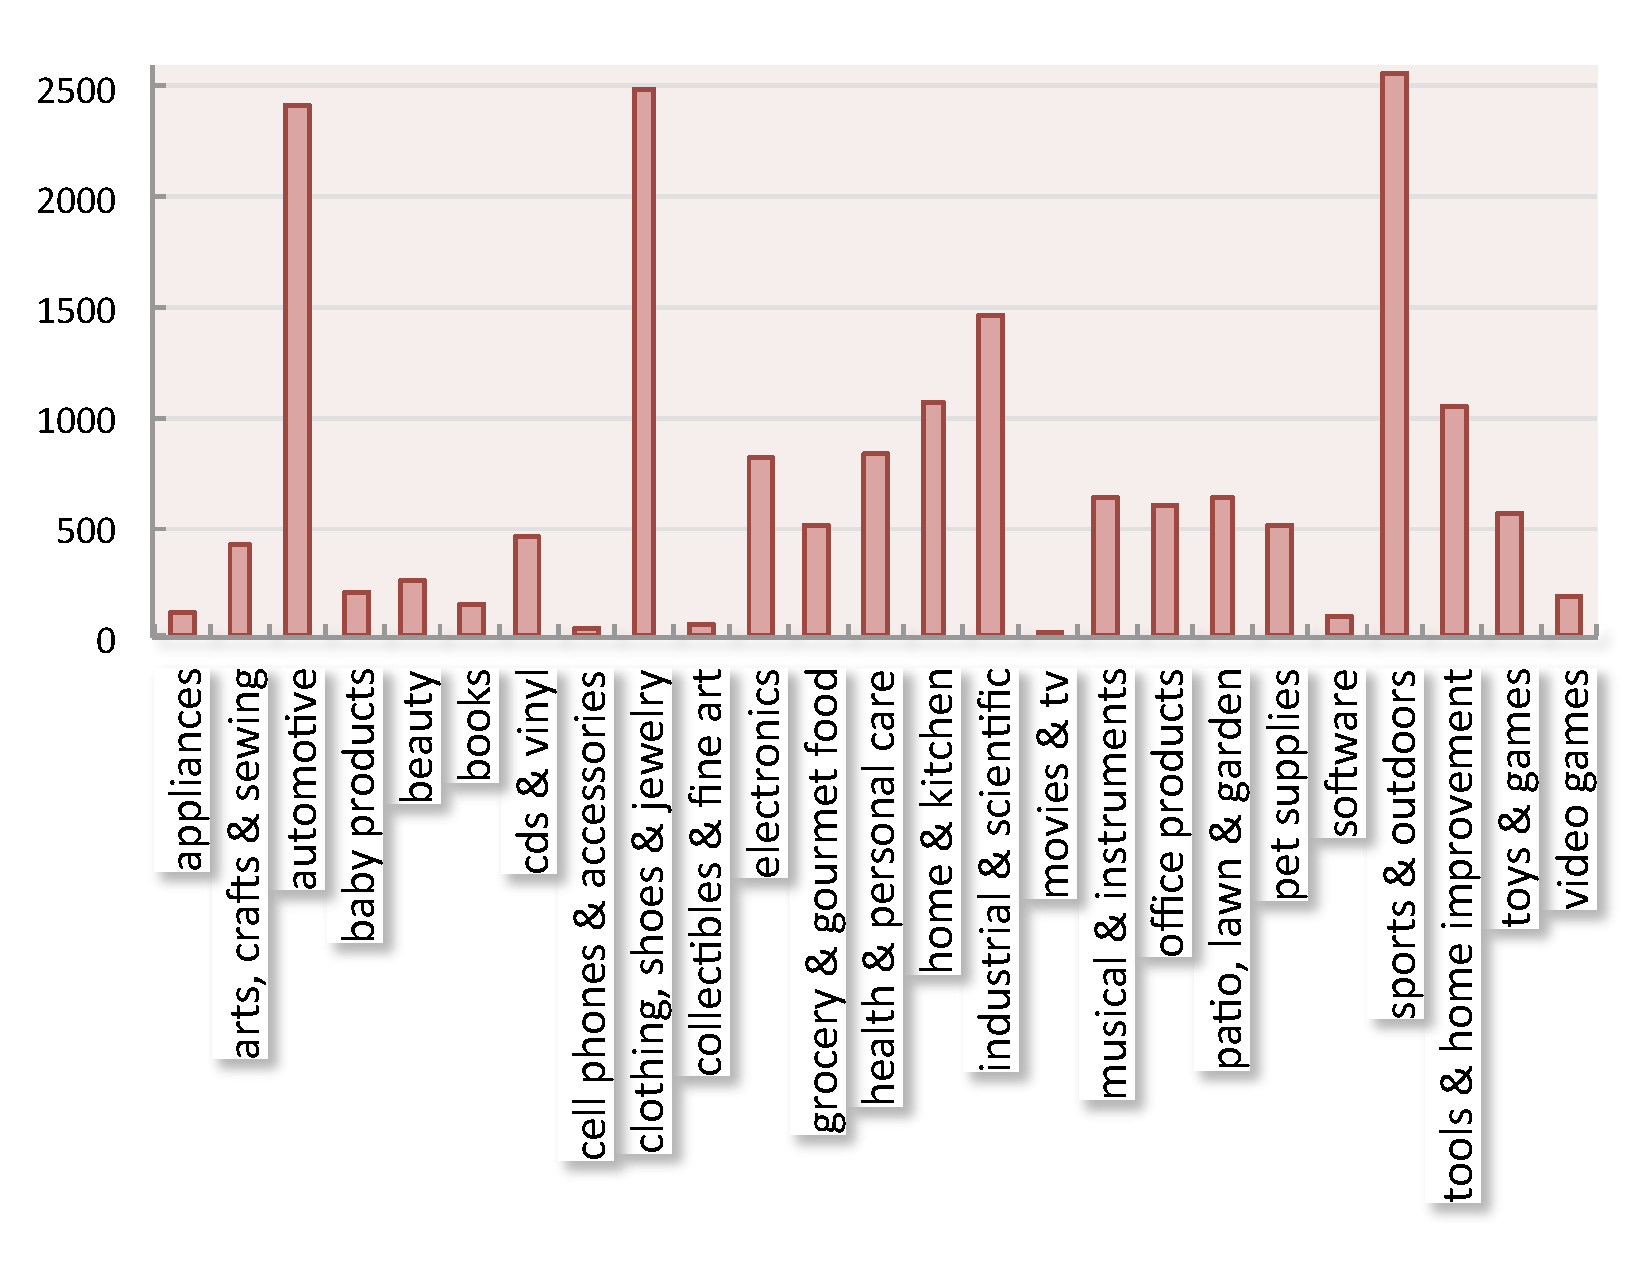
\includegraphics[width=0.33\textwidth]{images/amazonj-branches}} \hspace{0.01cm}
\subfloat[{BU2 branch stats}]{\label{Figure_BU2-branches}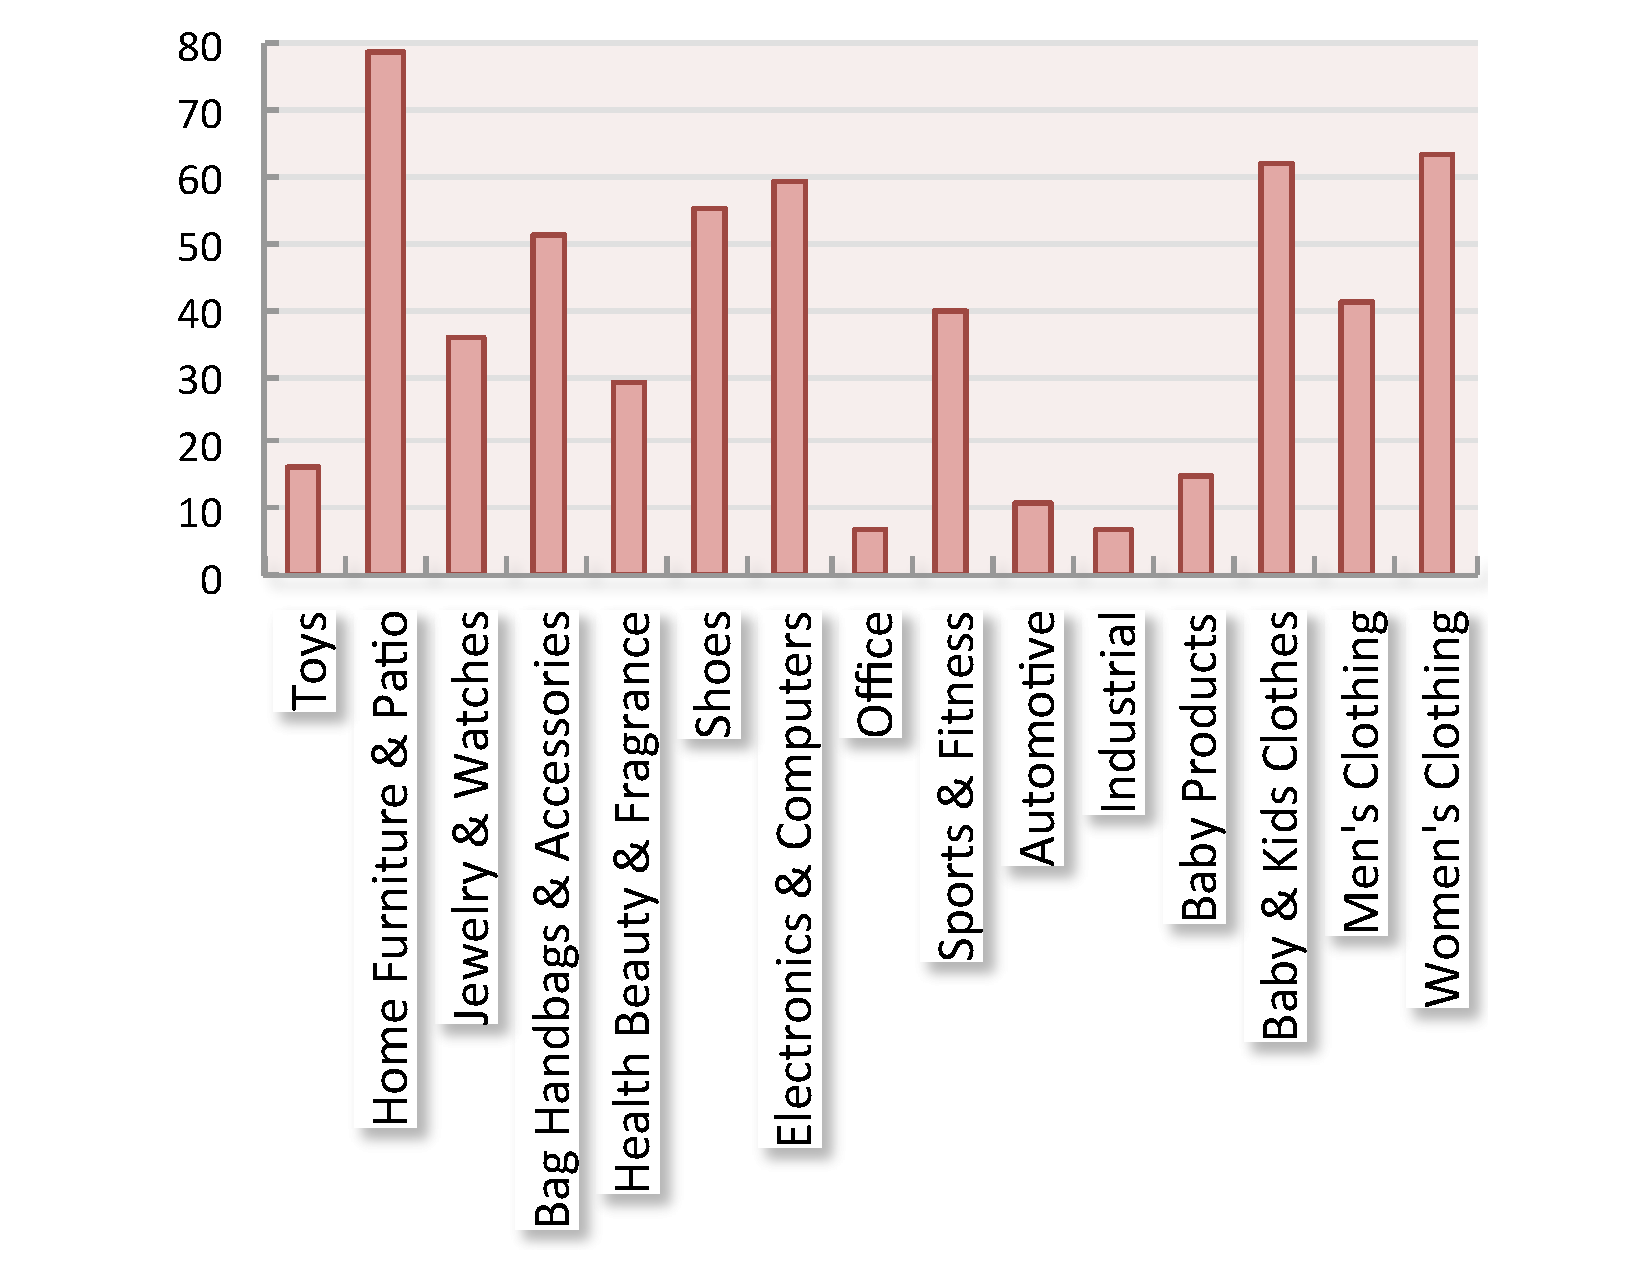
\includegraphics[width=0.32\textwidth]{images/BU2-branches}} \hspace{0.01cm}

\subfloat[{BU1 KL divergence}]{\label{Figure_BU1-KL}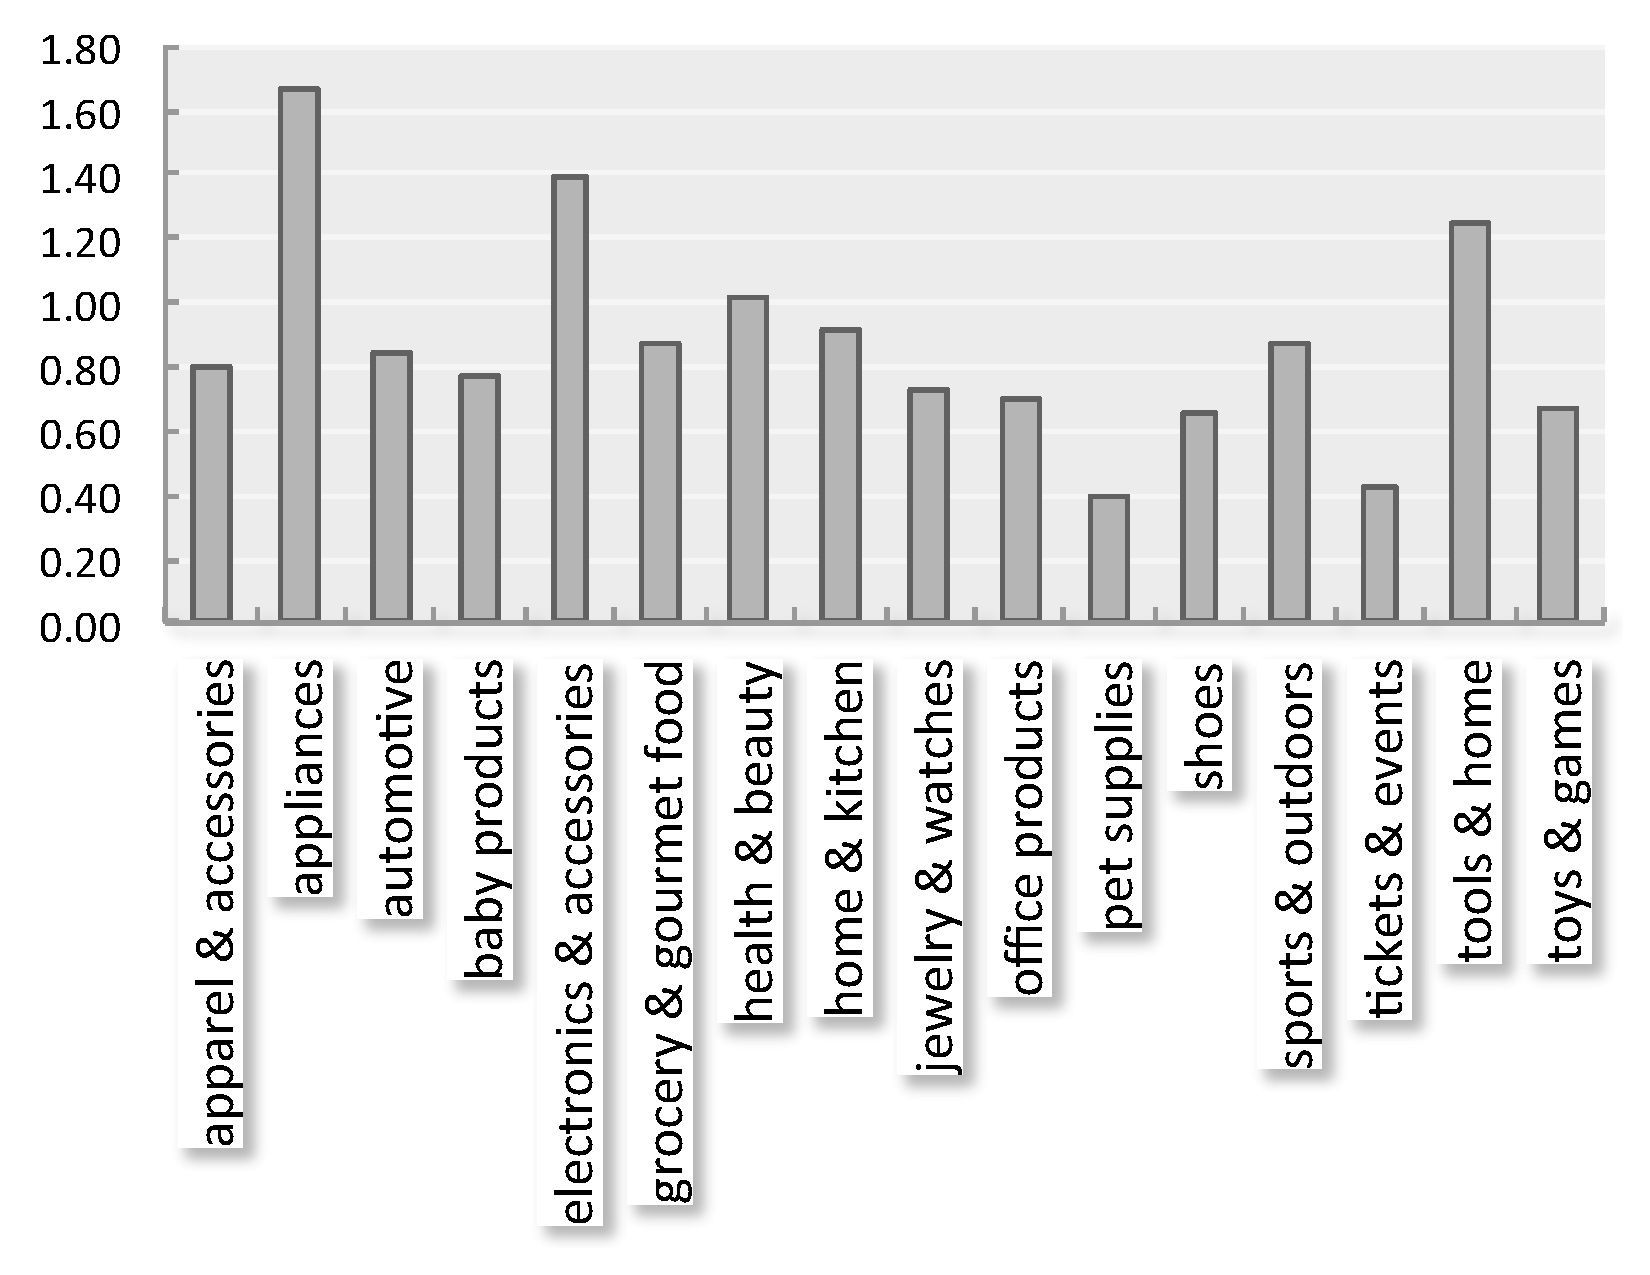
\includegraphics[width=0.31\textwidth]{images/BU1-KL}} \hspace{0.01cm}
\subfloat[{AmazonJulian KL divergence}]{\label{Figure_amazonj-KL}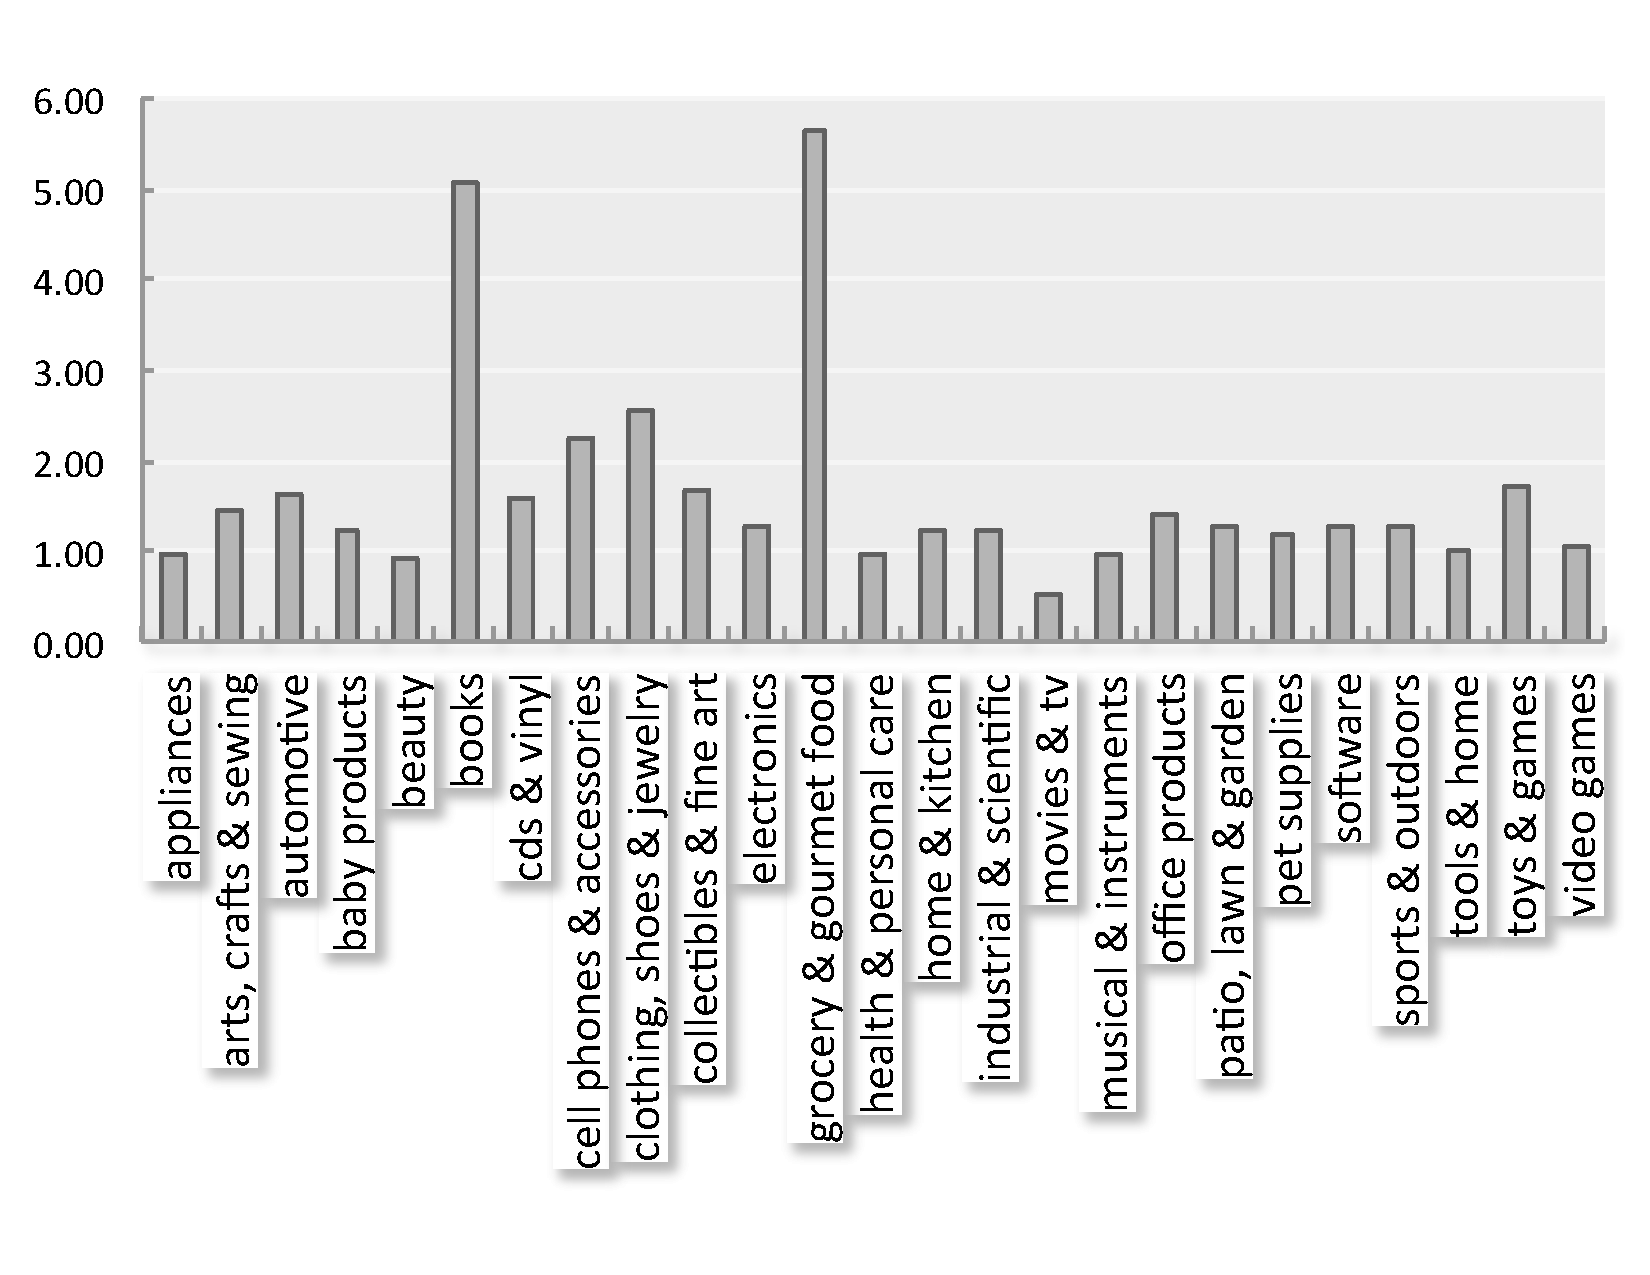
\includegraphics[width=0.33\textwidth]{images/amazonj-KL}} \hspace{0.01cm}
\subfloat[{BU2 KL divergence}]{\label{Figure_BU2-KL}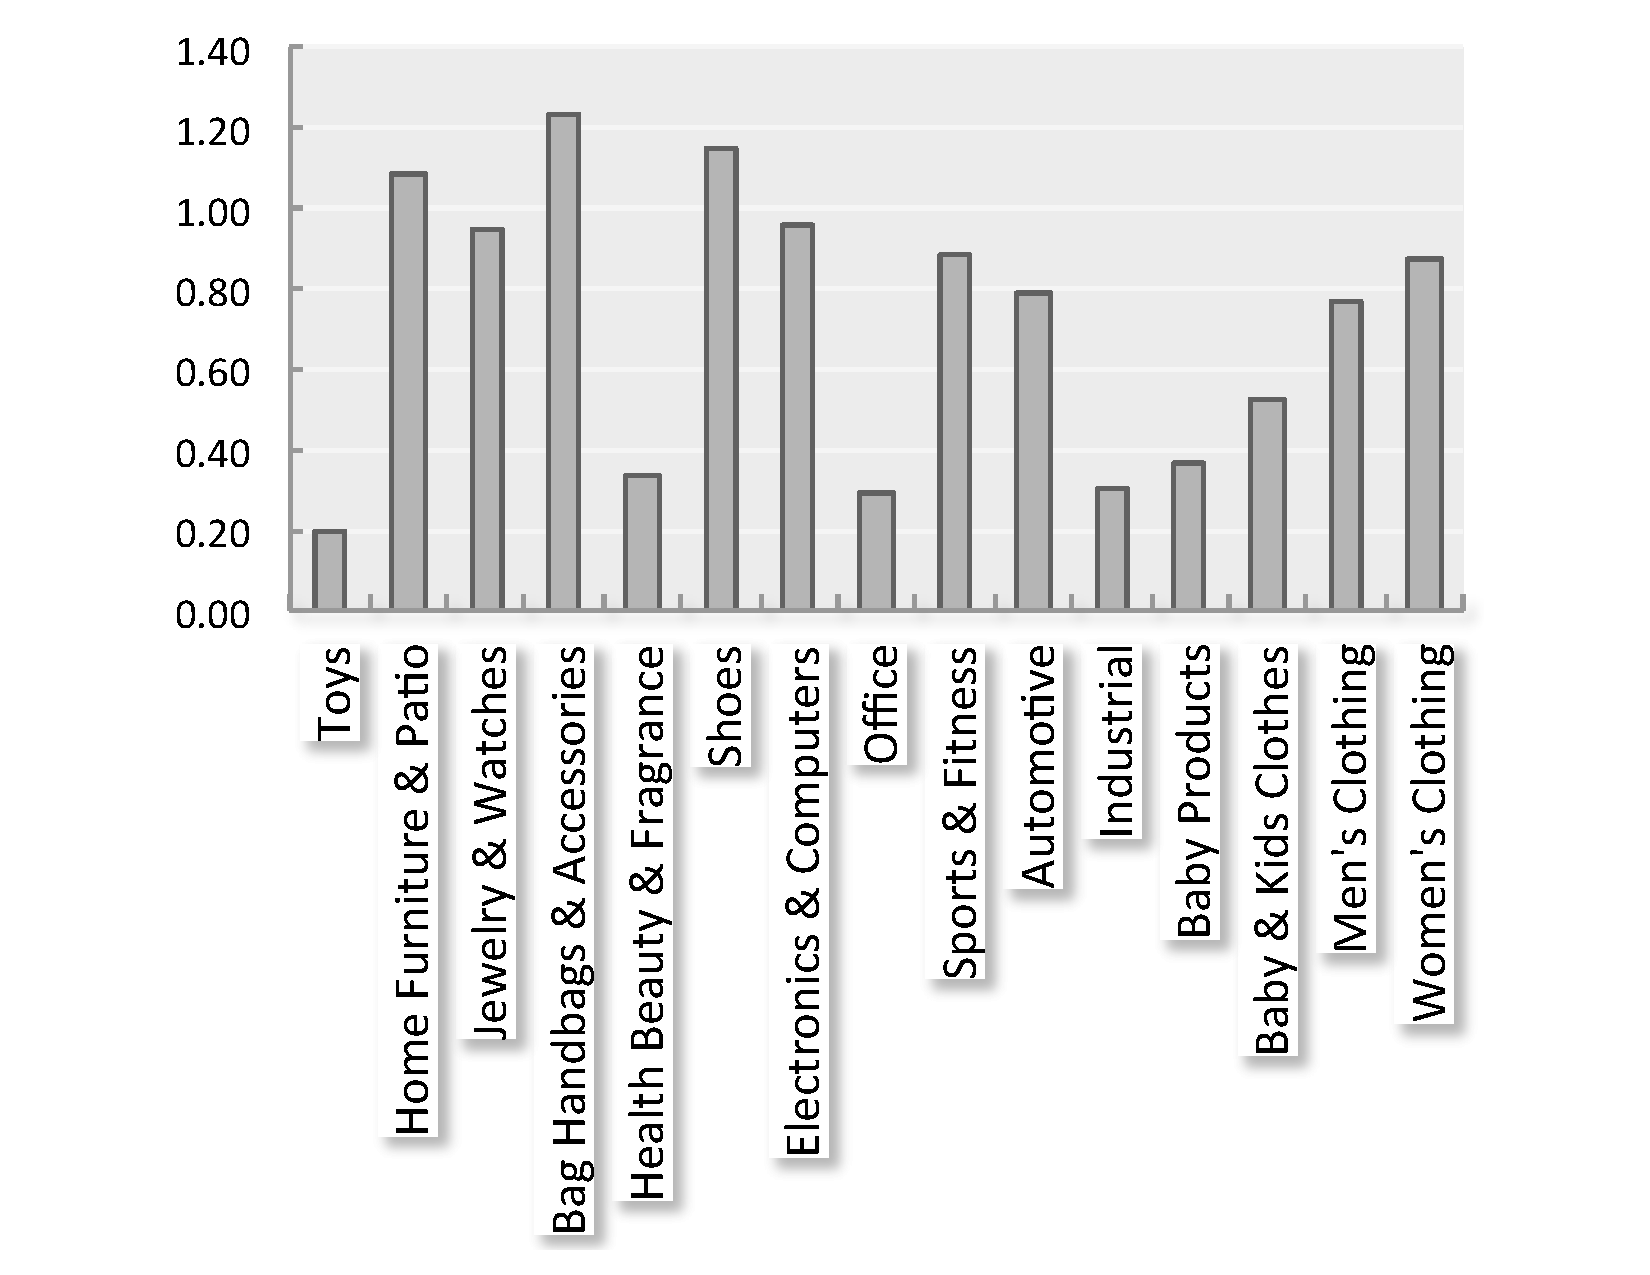
\includegraphics[width=0.31\textwidth]{images/BU2-KL}} \hspace{0.01cm}
\caption{{Dataset Statistics} }
\label{Figure_Dataset-statistics}
\end{figure}

\footnote{\scriptsize{\url{http://blog.salsify.com/root-cause-bad-ecommerce-site-search-company-behind-humble-barcode-trying-help}}}